\section{Auswertung}

Um die Extinktionsspektren zu erzeugen wurde das Ethanol/Ethanol Transmissionspektrum $\text{I}_{\text{Leer}}$ (siehe Abbildung \ref{fig:I_Leer}) jeweils durch die Transmissionsspektren $\text{I}_{\text{Substanz}}$, welche verschiedenen Konzentrationen des Kristallvioletts gelöst in Ethanol enthielten, dividiert und anschließend der dekadische Logarithmus aus dem Quotienten gebildet. Die erhaltenen Extinktionsgraphen wurden in Abbildung~\ref{fig:Extinktionalle} aufgetragen.


\begin{figure}[H]
	\centering	
	\begin{minipage}{1\textwidth}
	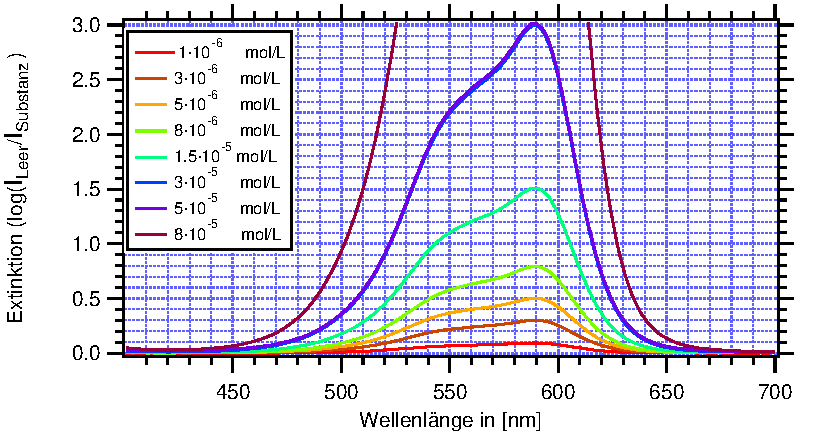
\includegraphics[width=\columnwidth]{Rohdaten/alleExtinktionenzusammen.pdf}	
	\caption{Extinktionen einer Kristallviolett/Ethanol Lösung verschiedener Konzentrationen. Die zugrundeliegenden Transmissionsmessungen wurden mit einem JASCO V-750 Spektrometer aufgenommen unter Verwendung von PMMA Küvetten mit einer Wegstrecke $L=10 \si{mm}$. Die Graphik wurde mit Igor Pro 6.37 erstellt.}
	\label{fig:Extinktionalle}
	\end{minipage}
	
\end{figure}
	


Aus den Extinktionen der Maxima (bei $589~\si{nm}$) der verschiedenen Konzentrationen konnte nach Gleichung \ref{linplot} der Graph in Abbildung \ref{linplot} erstellt werden, aus deren Steigung der dekadische Extinktionskoeffizient ermittelt werden konnte. Dieses wurde für 10 weitere Wellenlängen im Abstand von $10 \si{nm}$ wiederholt.